\documentclass{article}

% Language setting
% Replace `english' with e.g. `spanish' to change the document language
\usepackage[english]{babel}

% Set page size and margins
% Replace `letterpaper' with`a4paper' for UK/EU standard size
\usepackage[letterpaper,top=2cm,bottom=2cm,left=3cm,right=3cm,marginparwidth=1.75cm]{geometry}

% Useful packages
\usepackage{amsmath}
\usepackage{float}
\usepackage{graphicx}
\usepackage{amsmath}
\usepackage{hyperref}
\usepackage{cleveref}
\numberwithin{equation}{section}
\numberwithin{figure}{section}
\numberwithin{table}{section}
\numberwithin{table}{section}
\crefname{table}{Tab.}{Tab.}
\crefname{figure}{Fig.}{Fig.}
\crefname{equation}{Eq.}{Eq.}

\usepackage{sectsty}
\allsectionsfont{\sffamily}

\usepackage[dvipsnames]{xcolor}
\usepackage{tikz}
\usetikzlibrary{calc}
\usepackage{siunitx}
%\usepackage{anyfontsize}


\begin{document}
\thispagestyle{empty}%
\addtocounter{page}{-1}%
\begin{tikzpicture}[overlay,remember picture]

    % Background color
    \fill[
    black!2]
    (current page.south west) rectangle (current page.north east);
    
    % Rectangles
    \shade[
    left color=Dandelion, 
    right color=Dandelion!40,
    transform canvas ={rotate around ={45:($(current page.north west)+(0,-6)$)}}] 
    ($(current page.north west)+(0,-6)$) rectangle ++(9,1.5);
    
    \shade[
    left color=lightgray,
    right color=lightgray!50,
    rounded corners=0.75cm,
    transform canvas ={rotate around ={45:($(current page.north west)+(.5,-10)$)}}]
    ($(current page.north west)+(0.5,-10)$) rectangle ++(15,1.5);
    
    \shade[
    left color=lightgray,
    rounded corners=0.3cm,
    transform canvas ={rotate around ={45:($(current page.north west)+(.5,-10)$)}}] ($(current page.north west)+(1.5,-9.55)$) rectangle ++(7,.6);
    
    \shade[
    left color=orange!80,
    right color=orange!60,
    rounded corners=0.4cm,
    transform canvas ={rotate around ={45:($(current page.north)+(-1.5,-3)$)}}]
    ($(current page.north)+(-1.5,-3)$) rectangle ++(9,0.8);
    
    \shade[
    left color=red!80,
    right color=red!80,
    rounded corners=0.9cm,
    transform canvas ={rotate around ={45:($(current page.north)+(-3,-8)$)}}] ($(current page.north)+(-3,-8)$) rectangle ++(15,1.8);
    
    \shade[
    left color=orange,
    right color=Dandelion,
    rounded corners=0.9cm,
    transform canvas ={rotate around ={45:($(current page.north west)+(4,-15.5)$)}}]
    ($(current page.north west)+(4,-15.5)$) rectangle ++(30,1.8);
    
    \shade[
    left color=RoyalBlue,
    right color=Emerald,
    rounded corners=0.75cm,
    transform canvas ={rotate around ={45:($(current page.north west)+(13,-10)$)}}]
    ($(current page.north west)+(13,-10)$) rectangle ++(15,1.5);
    
    \shade[
    left color=lightgray,
    rounded corners=0.3cm,
    transform canvas ={rotate around ={45:($(current page.north west)+(18,-8)$)}}]
    ($(current page.north west)+(18,-8)$) rectangle ++(15,0.6);
    
    \shade[
    left color=lightgray,
    rounded corners=0.4cm,
    transform canvas ={rotate around ={45:($(current page.north west)+(19,-5.65)$)}}]
    ($(current page.north west)+(19,-5.65)$) rectangle ++(15,0.8);
    
    \shade[
    left color=OrangeRed,
    right color=red!80,
    rounded corners=0.6cm,
    transform canvas ={rotate around ={45:($(current page.north west)+(20,-9)$)}}] 
    ($(current page.north west)+(20,-9)$) rectangle ++(14,1.2);
    
    % logo
    \node[midway,right=5.5cm,yshift=-10.8cm]
    {
    
\includegraphics[scale=0.15]{cover/LogoMuner.png}
    };
    
    % Title
    \node[align=center,yshift=-40pt] at ($(current page.center)+(0,-5)$) 
    {
    {\fontsize{25}{32} \selectfont {{Citycar comfort evaluation, comparing suspension}}
    }\\[2pt]
    {\fontsize{25}{32} \selectfont {{in case of traditional and In-wheel powertrain}}
    }\\[1cm]
    {\fontsize{16}{19.2} \selectfont \textcolor{orange!80!black}{ \bf R.La Rocca, J.Ferretti}}\\[3pt]
    Dynamics and Compliant Control of Electric Vehicles\\[3pt]
    A.Y. 2020/2021};
    \end{tikzpicture}
\newpage
\tableofcontents
\newpage
%%%%%%%%%%%%%%%%%%%%%
\section{Introduction}
The following report is focused on the suspension analysis of a very famous Italian citycar, the FIAT 500, in the newest electric powertrain configuration. Two different powertrain were analyzed, the first one is the classical one with the motor inside the body of the car. The second one consider an hypothetical configuration with the motor inside the wheel: a possibility that can be applied only in in electric vehicles.

\begin{figure}[H]
    \centering
    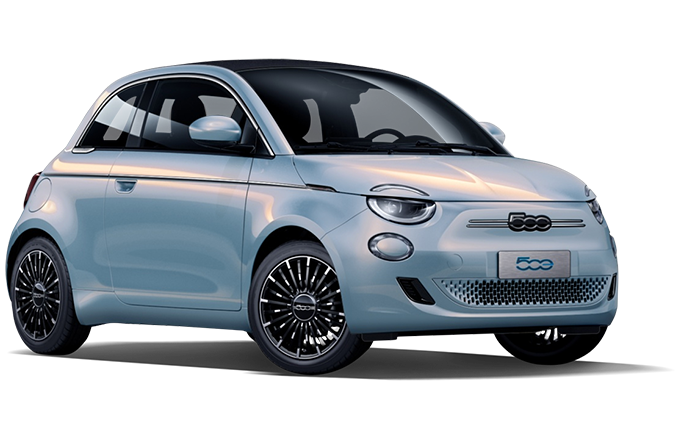
\includegraphics[width=0.6\textwidth]{Pictures/fiat 500e.png}
    \caption{\emph{FIAT 500e}}
    \label{fig:1}
\end{figure}

One of the main objective of the suspension in this type of cars is to guarantee a good level of comfort to the passenger. %a quarter car model was implemented using the software Activate from Altair.\\
In the second chapter the characteristics of the vehicle are reported with a focus on the used suspension type and on the characteristics of the In-wheel electric motor chosen for the hypothetical configuration.\\
In the third chapter are reported the theoretical advantage and disadvantage of the In-wheel configuration, highlighting the possible vehicle dynamics problems related to the increase of the unsprung mass due to the motor inside the wheel.\\
In the last chapters the model and the results of the simulation are presented for both the vehicles configuration. The vehicles were simulated with both passive and active suspension. An optimazer was implemented to obtain better values for both PID parameters (Kp,Ki,Kd) and for the suspension datas (ks and cs).

\subsection{Aim of the analysis}
A suspension system in a vehicle aims to provide both comfort, for passengers, and road handling, for the driver. The focus of this report is the comfort of the passengers, so the ability of the vehicle to insulating passengers from vibrations caused by roads.\\
The excess of vibration can have an impact also on the human health, for this reason vertical acceleration must be minimized and oscillation must be attenuated.


\section{Vehicle characteristics}
In the following chapter the characteristics and the parameters of the FIAT 500e and the In-wheel motor are reported.

\subsection{Fiat 500e}
The FIAT 500e is one of the latest model presented in 2020 by the Italian manufacturer and the first one with a dedicated BEV configuration (In 2013 it was made an electric conversion of the internal combustion engine version).\\
With a total length of \SI{3632}{\milli\metre} and a width of \SI{1683}{\milli\metre} and an estimated range of \SI{320}{\kilo\metre}, this car is a perfect citycar and possible good option for the sharing car companies.

\subsubsection{Suspension type}
The FIAT 500e use an Independent McPherson for the front suspension and a Semi-independent suspension in the rear wheels.

\begin{figure}[H]
\centering
\begin{minipage}{.5\textwidth}
  \centering
  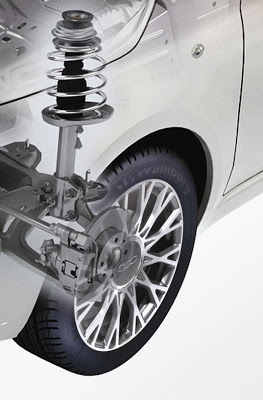
\includegraphics[width=.4\linewidth]{Pictures/Fiat500USA-Fiat 500 front suspension.png}
  \caption{\emph{FIAT 500 front suspension}}
  %\captionof{figure}{A figure}
  \label{fig:2}
\end{minipage}%
\begin{minipage}{.5\textwidth}
  \centering
  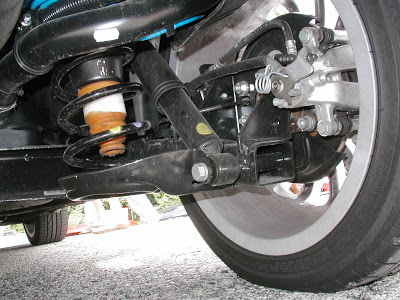
\includegraphics[width=.8\linewidth]{Pictures/Fiat500USA-500_RR_without_Saybar.jpg}
  \caption{\emph{FIAT 500 rear suspension}}
  %\captionof{figure}{Another figure}
  \label{fig:3}
\end{minipage}
\end{figure}
In \cref{fig:2} and \cref{fig:3} the details of the suspensions of the FIAT 500 with the internal combustion engine, we suppose that in the electric version this configuration is more or less the same.\\
Both front and rear suspension are \emph{Passive} systems made up of mechanical elements, springs and dumpers. The spring can be compressed or extended, this allow to contrast the disturbance forces acting on the system. The dumper works against the spring displacement, in order to damp the oscillations.\\
This type of suspension is able only to react passively to an external force, damping and stiffness coefficient are chosen in order to ensure good performance in both comfort and handling. The chosen parameters are fixed and they can change only due to aging of components that decrease the performances.\\
\newline
In the following quarter car models will be considered only the front suspension, in both classic and In-wheel configuration. The values chosen for the stiffness of sprung \emph{(ks)} is 30000 and for the dumping of sprung \emph{(cs)} is 3000. 


\subsubsection{Tires and Rims size}
The FIAT 500e use 15" wheel rims with a size of 185/65 for the tires. The tire stiffness \emph{(kus)} is not easy to find but after some research we supposed that 200000 is a good approximation. The data will be the same for both the vehicle configuration.

\subsection{FIAT 500e motor}
What does move the FIAT 500e is a 3-phase permanent magnet synchronous motor which has the following characteristics:
\begin{table}[H]
    \centering
    \begin{tabular}{|c|c|}
        \hline
        Maximum Power& \SI{88}{\kilo\watt}\\
        \hline
        Weigt & \SI{60}{\kilo\gram}\\
        \hline
        Maximum Torque & \SI{220}{\newton\metre}\\
        \hline
        Maximum speed & \SI{250}{\kilo\metre/\hour}\\
        \hline
        0-100 accelleration & \SI{9}{\second}\\
        \hline
    \end{tabular}
    \caption{500e motor specification}
    \label{tab:my_label}
\end{table}
For a small citycar like those specs are more than enough, and the weight of \SI{60}{\kilo\gram} is a great achievement.\\
\begin{figure}[H]
    \centering
    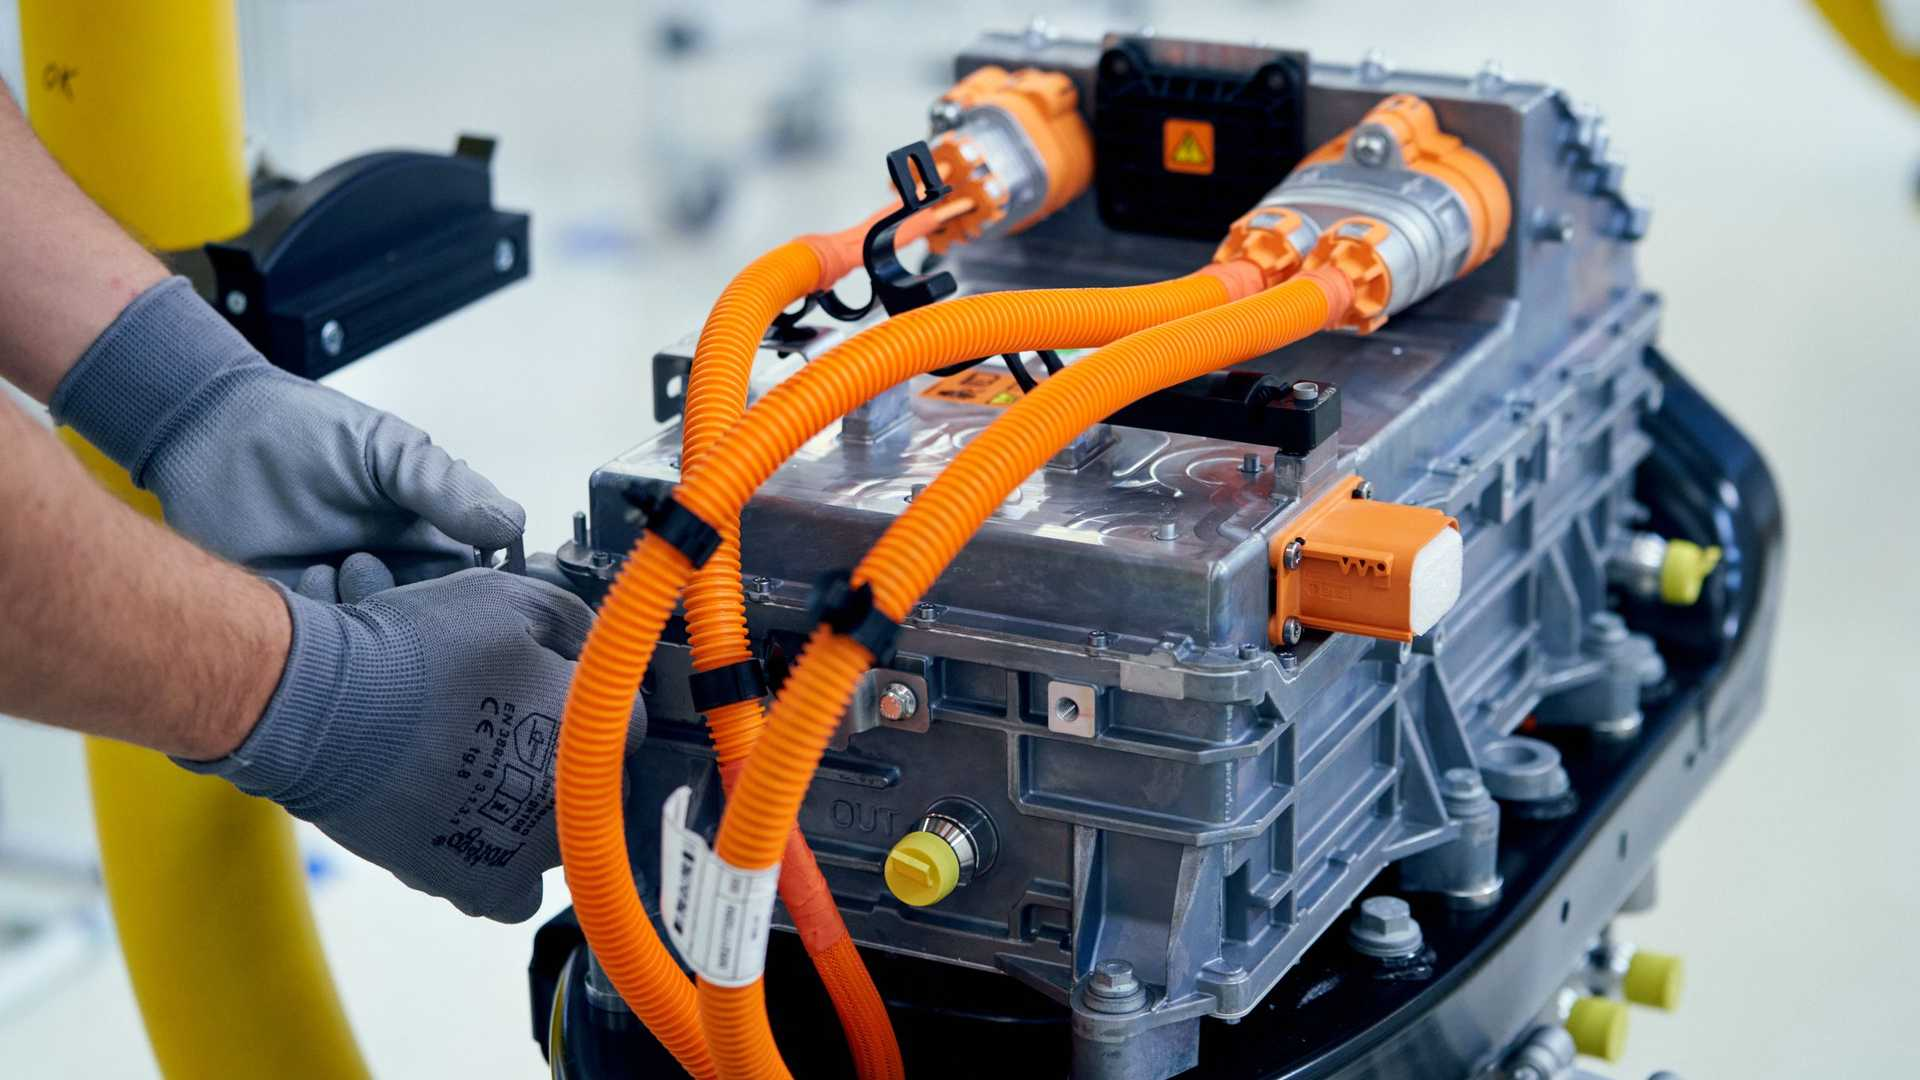
\includegraphics[width=0.6\textwidth]{Pictures/500e_motor.jpg}
    \caption{\emph{FIAT 500e powertrain}}
    \label{fig:500e_motor}
\end{figure}
From what you can see in \cref{fig:500e_motor}, its volumetric size is comparable to the ICE counterpart, so it can be easily fitted under the front hood.
\subsection{In-wheel motor}
A different approach to the classic "single" power train configuration, is to use a "network" of 2 or more motors coupled together, this will let us split the power flow during the vehicle running.\\
On the current state of the art of e-motors, an interesting solution is to use an \emph{In-wheel motor}:\\
Those are "wheel shaped" motors to be mounted directly on the wheel hub, removing many mechanical parts like the Cardan joint.\\
There are many advantages of using the in-wheel motor:
\begin{itemize}
    \item \textbf{More energy efficiency:} for example the the Cardan joint and the differential are removed (the efficiencies of those component in a single motor configuration are approximately $\eta_c=99\%$ and $\eta_d=95\%$).
    \item \textbf{Cost and Weight saving:} as said before, we will have less mechanical parts to use.
    \item \textbf{More freedom for control algorithm:} Torque vectoring control becomes simpler to be implemented, this is true for other safety related control systems such as ABS.
\end{itemize}
Those welcome advantages are followed by some drawbacks:
\begin{itemize}
    \item \textbf{More vibrations}: the motor now is more coupled to the asphalt, and vibrations could decrease its long term durability.
    \item \textbf{Isolation:} the wheels (and thus the motors) are more exposed tho the action of external agents like whater, mud, stones etc...
    \item \textbf{Higher propensity to structural failure} due to the direct exposition with the extern.
    \item \textbf{Increasing of the unsprung mass.} 
\end{itemize}
\underline{This increasing of the unsprung mass is what we will focus on in this paper}, we will point out how this can eventually become a problem for the vehicle handling, and if we can do something about it by using active suspensions.
\subsection{Elaphe M700}
\begin{figure}[H]
    \centering
    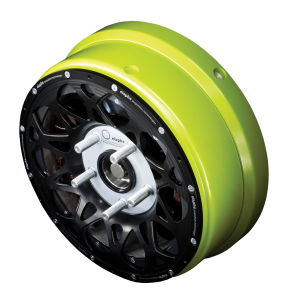
\includegraphics[width=0.3\textwidth]{Pictures/M700.png}
    \caption{\emph{Elaphe M700 in-wheel motor}}
    \label{fig:m700_motor}
\end{figure}
The In-Wheel motor chosen to our analysis is the Elaphe M700\cite{elapheM700_page}, it fits well on the 15" wheel rims of the FIAT 500, and if we use 2 motor configuration the car will reach approximately the same motor specification of the standard FIAT 500e.
In \cref{tab:m700_characteristics}, the characteristics of both the M700 and our 2-motor configuration.
\begin{table}[H]
    \centering
    \begin{tabular}{|c|c|c|}
        \hline
        & \textbf{1-motor}&\textbf{2-motors}\\
        \hline
        \hline
        Peak power& \SI{75}{\kilo\watt}&\SI{150}{\kilo\watt}\\
        \hline
        Continuous power& \SI{50}{\kilo\watt}&\SI{100}{\kilo\watt}\\
        \hline
        Weight& \SI{23}{\kilo\gram}&\SI{46}{\kilo\gram}\\
        \hline
    \end{tabular}
    \caption{Elaphe M700 characteristics}
    \label{tab:m700_characteristics}
\end{table}
As you can see from \cref{tab:m700_characteristics}, the total weight of the wanted configuration is \SI{46}{\kilo\gram}, that is even lower than the original FIAT 500e motor.

\section{Unsprung and Sprung mass}
If we look inside the quarter car model we see that it is possible to model a car with few parameters, two of them are the Unsprung and Sprung mass. By definition, the \emph{unsprung mass (mus)}  is the not suspended mass of a vehicle (wheels, tyres, part of the suspensions structure, brakes, hubs, bearings), while the \emph{sprung mass (ms)} is the remaining part of the vehicle (chassis, engine, passengers).\\ 
In the classical vehicle configuration the engine is part of the sprung mass, because it is placed inside the chassis, but in the second we find the motor inside the wheel. %In this report we are focusing in two types of configuration, one is the classical but in the second we find the motor inside the wheel. 
For this reason, from a model point of view, we have a shift of the mass of the engine from the Sprung to Unsprung mass.\\
This solution, of course, presents both advantages and disadvantages from the point of view of the electrical and mechanical implementation. The aim of this report is to evaluate the dynamics performance of a suspension system, and for this reason only this aspect will be investigated, highlighting the possible results obtained from an increase of the Unsprung mass.\\
\newline
From a theoretical point of view increase the unsprung mass leads to worst performances. In details:
\begin{itemize}
    \item \textbf{Higher vertical acceleration} that reduce the comfort of a vehicle.
    \item \textbf{Decrease the Handling ability}.
    \item \textbf{Unsprung components are harder to accelerate/decelerate} and thus it is more difficult for the suspension to maintain a consistent tire load.
    \item \textbf{Higher tire momentum}, that request higher torque to be controlled.
\end{itemize}
In general, for the unsprung mass, less is better. Less weight means less deformation of the springs and less shocks to control, the wheels can respond to the road faster and the suspension can keep the tyres in contact with the road. Another advantage is that passenger comfort improves.\\

\section{Model and Results}
The used model and the obtained results are shown in this section. A brief explanation of the quarter car model is followed by the parameters used to model both the configuration of vehicles.\\
\subsection{Software and enviroment}
The software used was Altair Activate\cite{altair_activate}: a Multi-disciplinary System Simulation that let us create models trough a simple but powerful GUI.\\
The results obtained from the model implementation with Altair Activate will be shown with a focus in the tuning of some parameters using an optimizer function.

\begin{figure}[H]
    \centering
    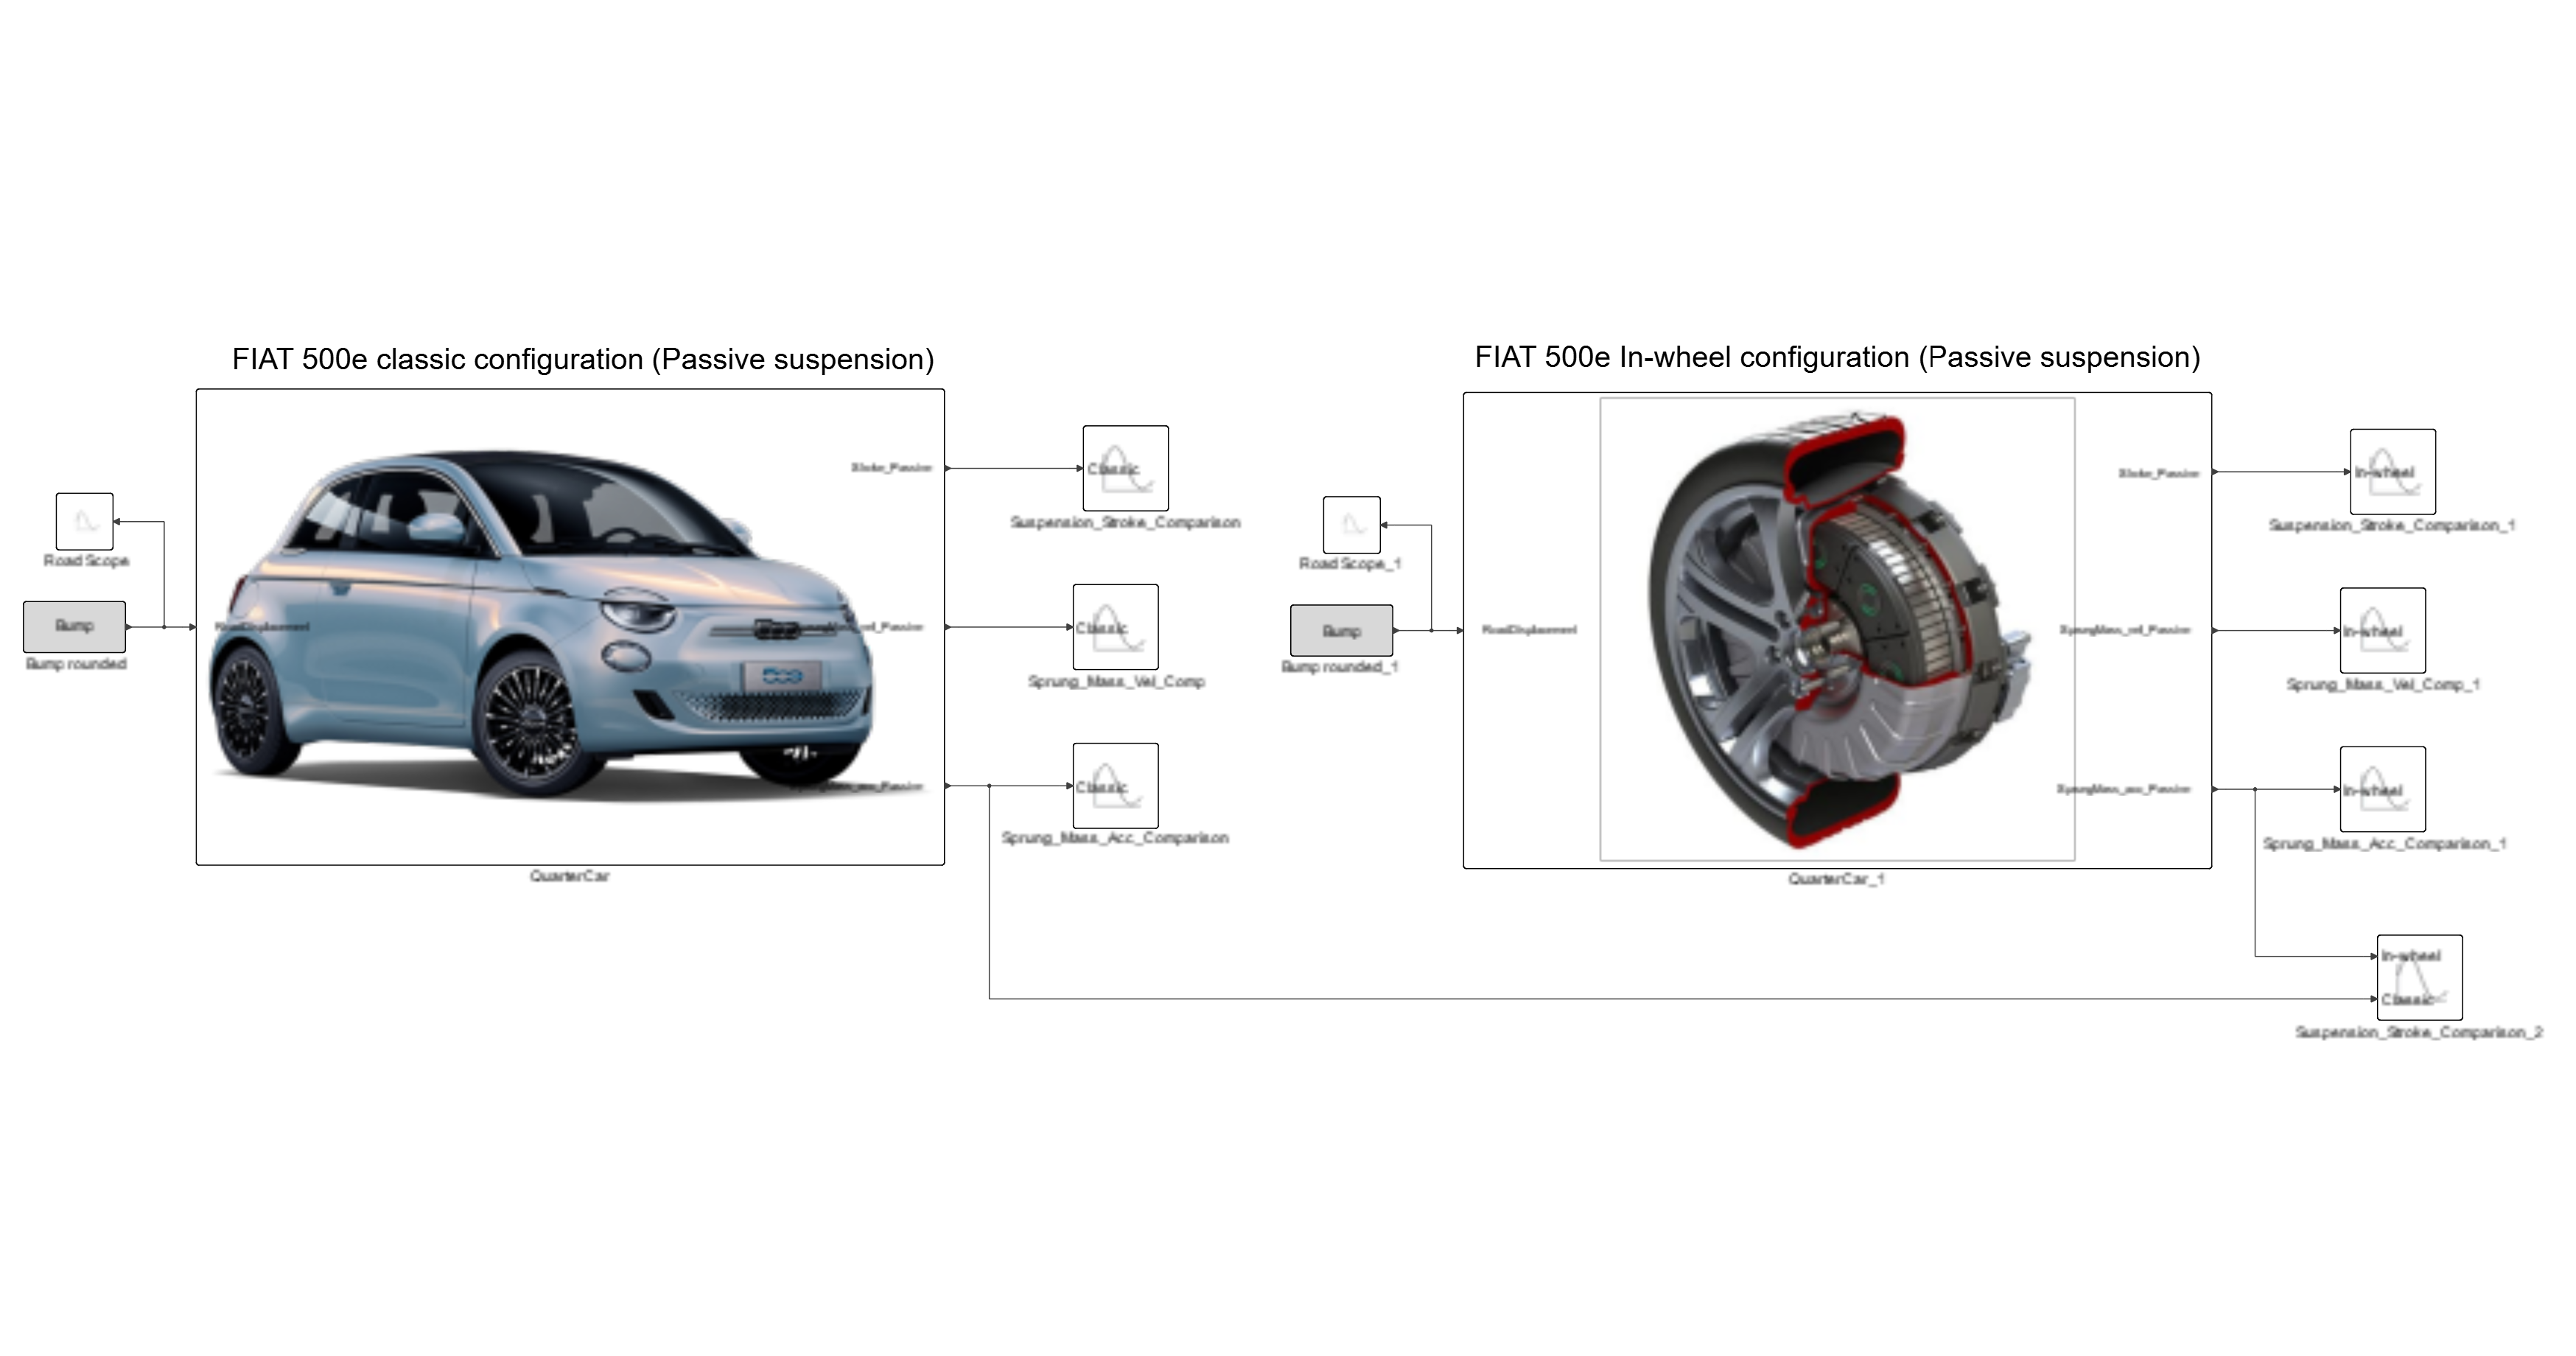
\includegraphics[width=1\textwidth]{Pictures/Models.png}
    \caption{\emph{Model implementation in Altair Activate}}
    \label{fig:Model}
\end{figure}

\begin{figure}[H]
    \centering
    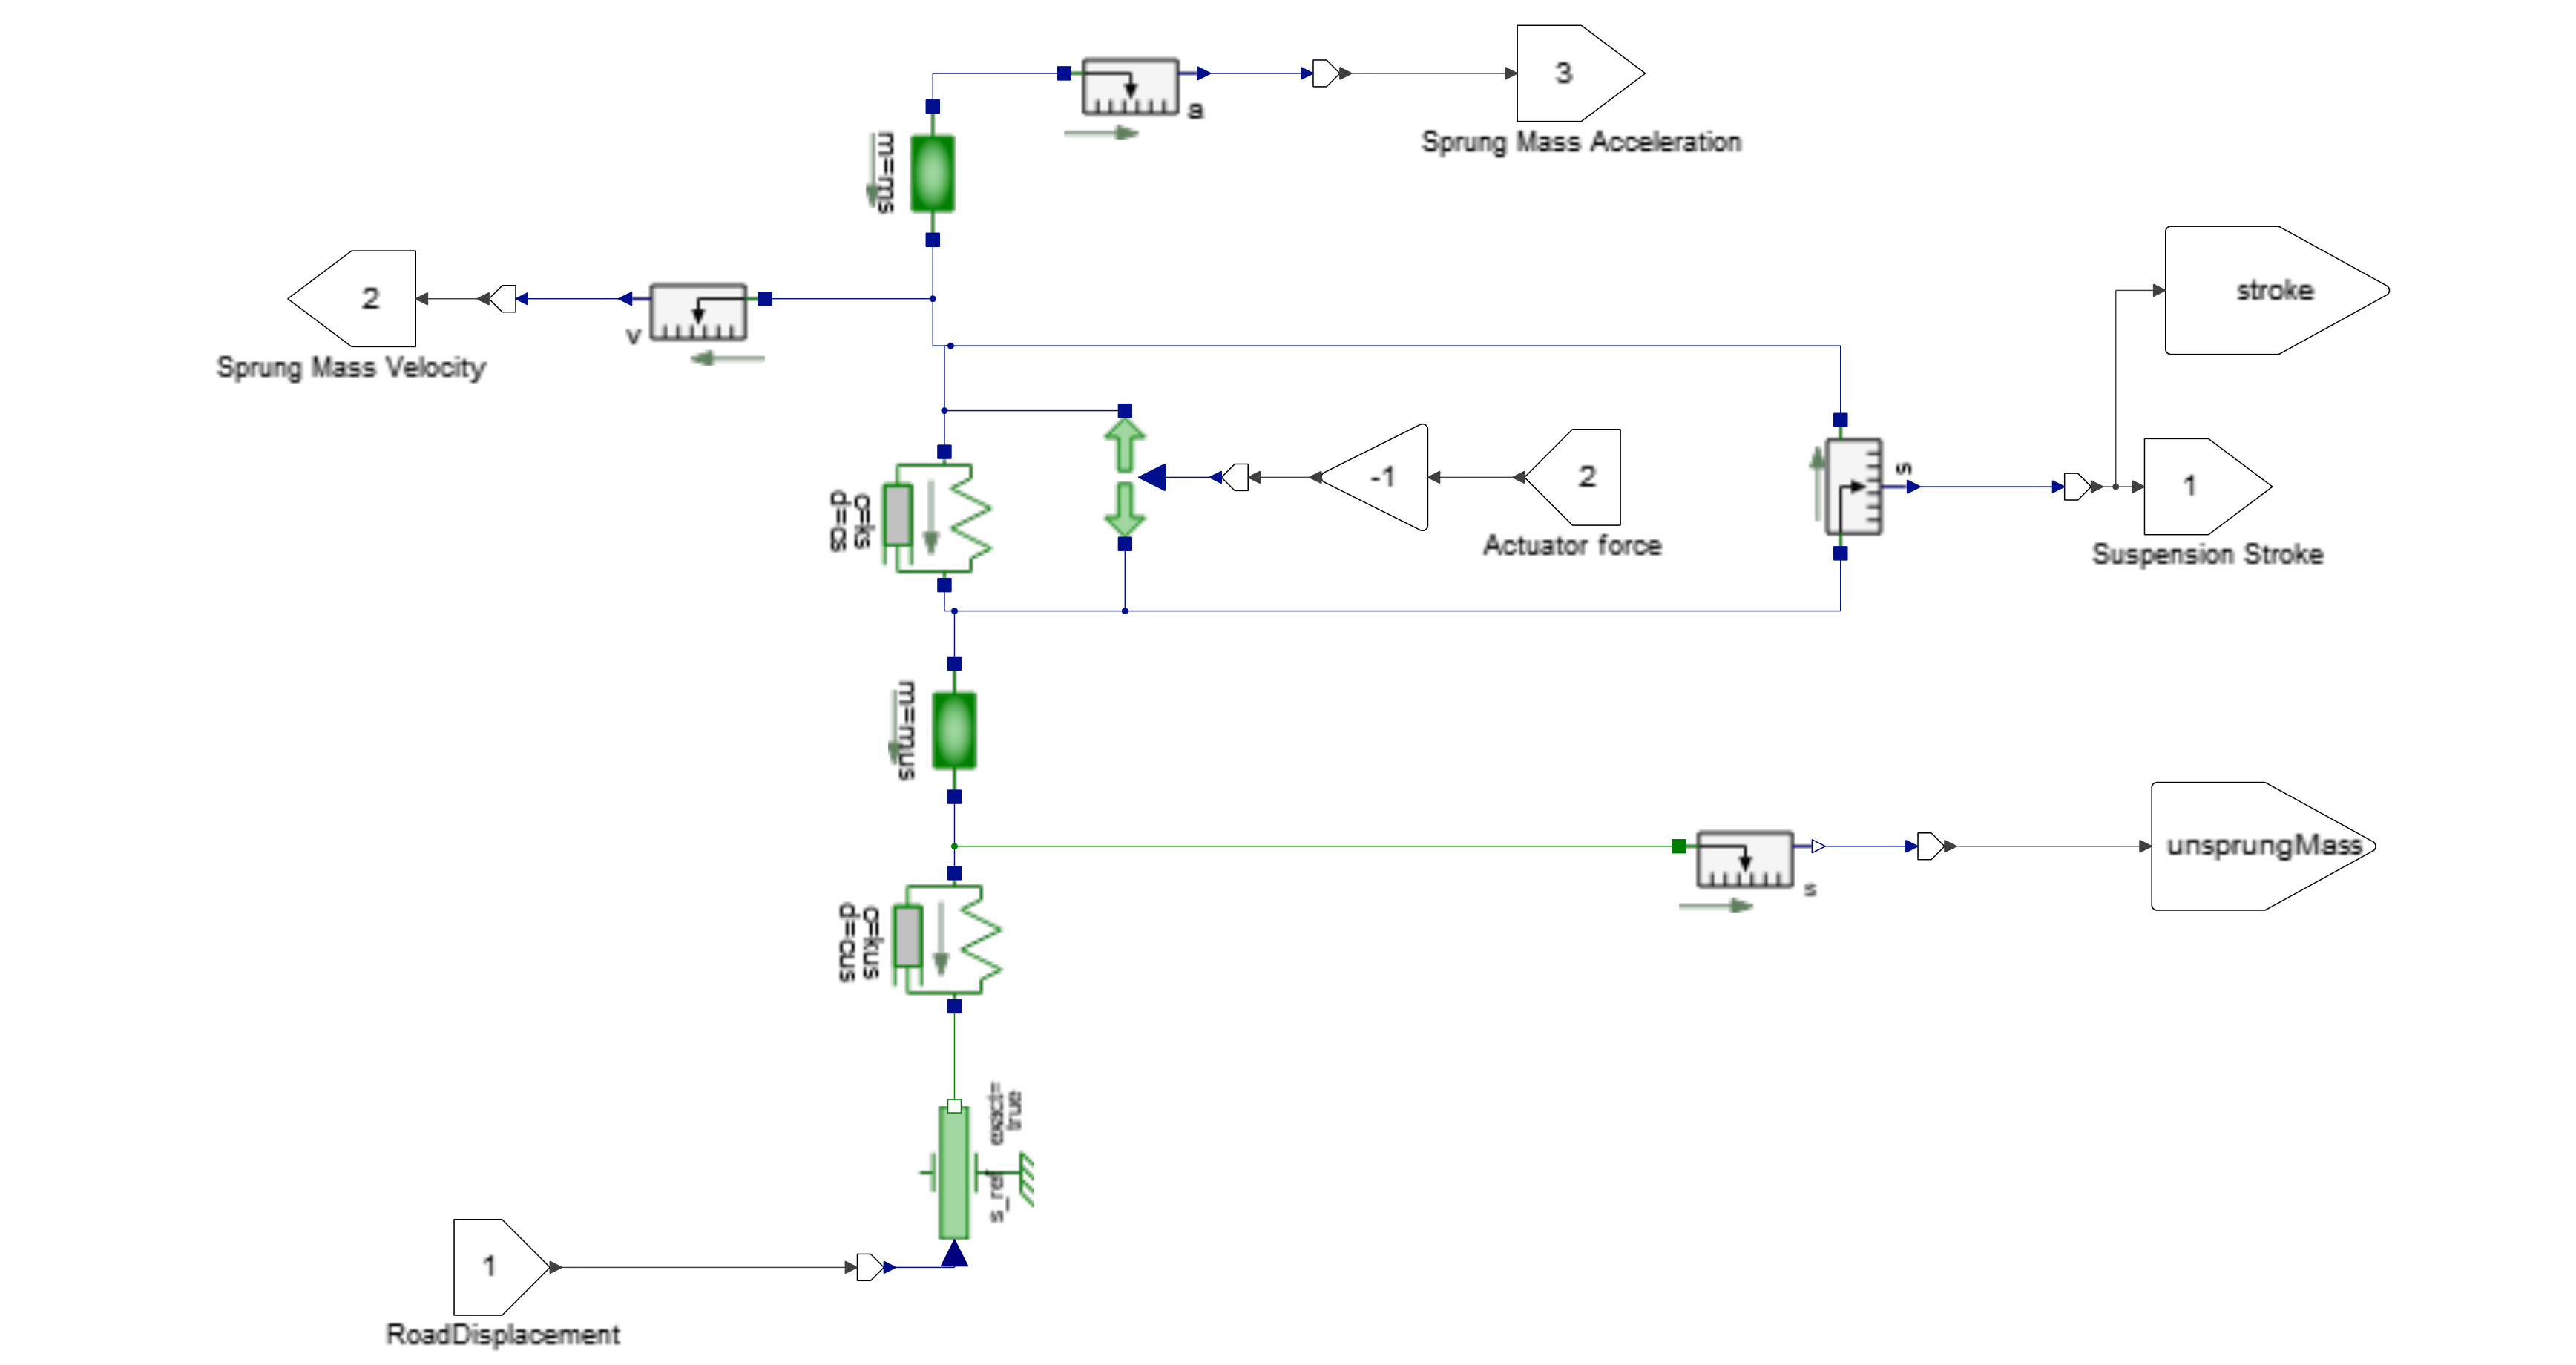
\includegraphics[width=0.8\textwidth]{Pictures/Quarter car model.png}
    \caption{\emph{Quarter car model implementation in Altair Activate }}
    \label{fig:Quarter car}
\end{figure}

\subsection{Road profile model}
In order to have a reliable simulation, we focused on creating a trustworthy road profile. The used profiles are two: a main bump created with the help of the professor, and a second one that try to recreate a more realistic profile of a road.
\subsubsection{profile \#1: big bump}
The first road profile modelled is a single bump with the height of \SI{0.1}{\metre} and the duration of \SI{0.2}{\second}. The profile was made by using a signal generator block, and a transfer function in series that introduce a time constant of $\tau=\SI{10}{\milli\second}$.
\begin{figure}[H]
\centering
\begin{minipage}{.55\textwidth}
  \centering
  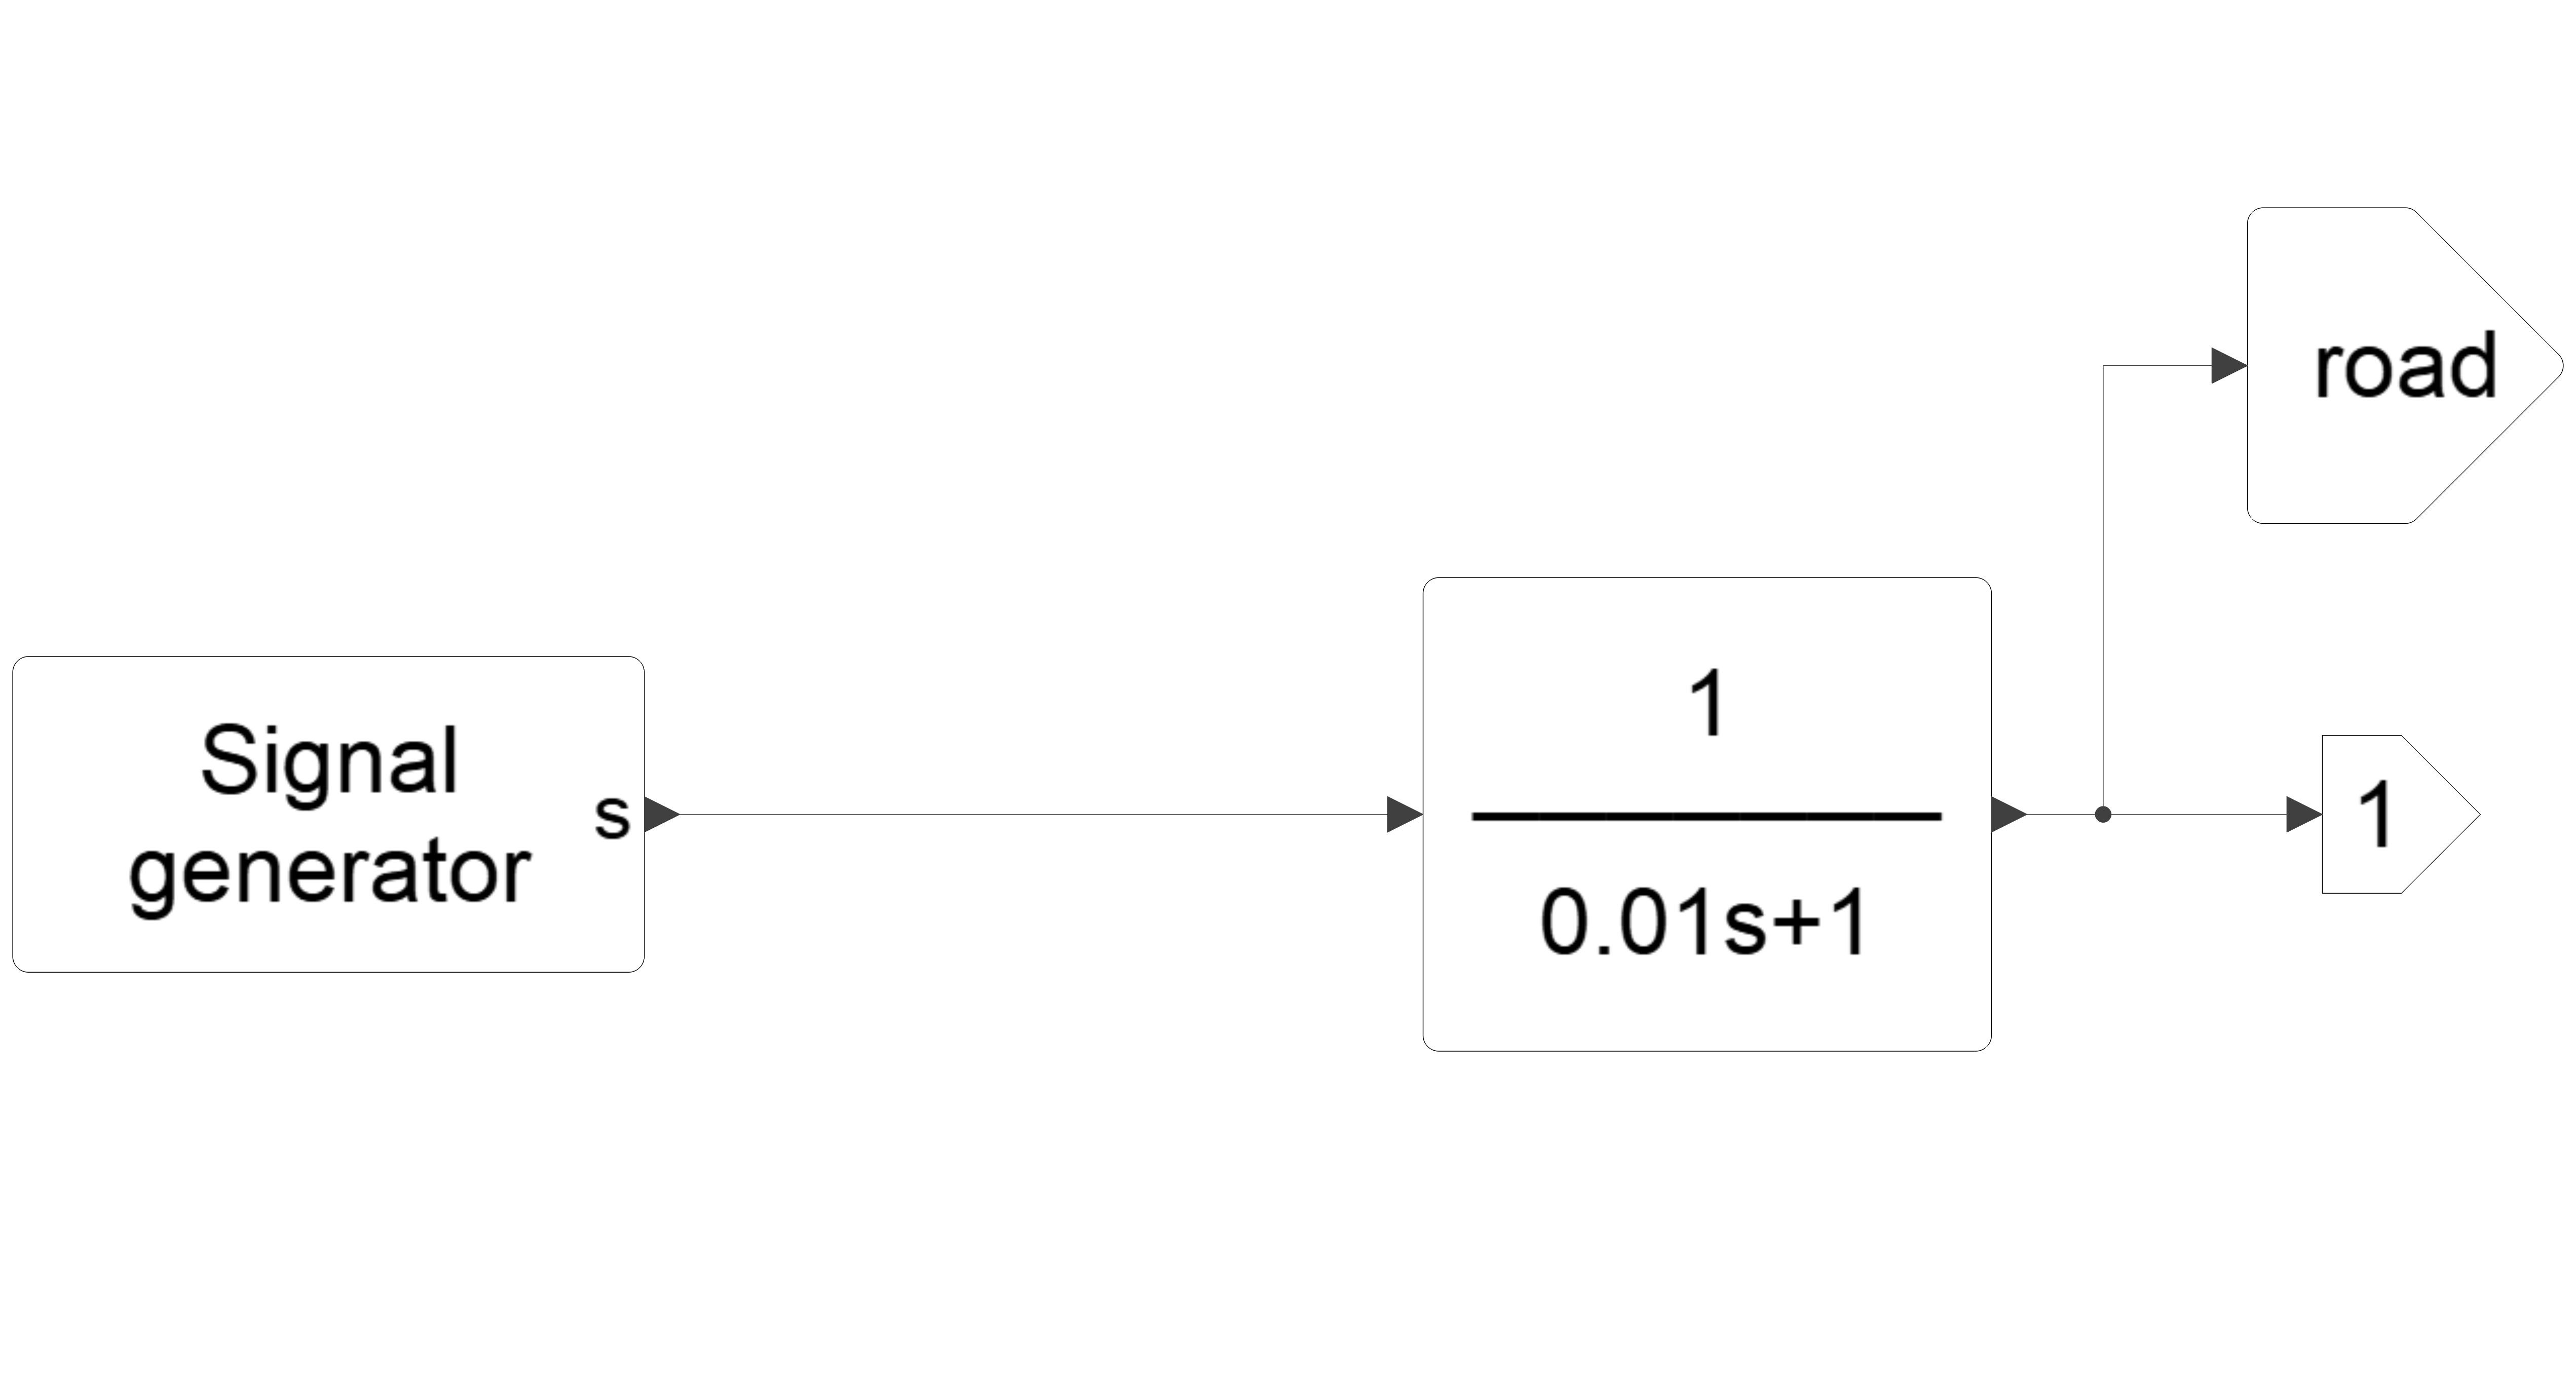
\includegraphics[width=.9\linewidth]{Pictures/big_bump_model.png}
  \caption{\emph{Road profile \#1 model}}
  %\captionof{figure}{A figure}
  \label{fig:1bump_model}
\end{minipage}%
\begin{minipage}{.45\textwidth}
  \centering
  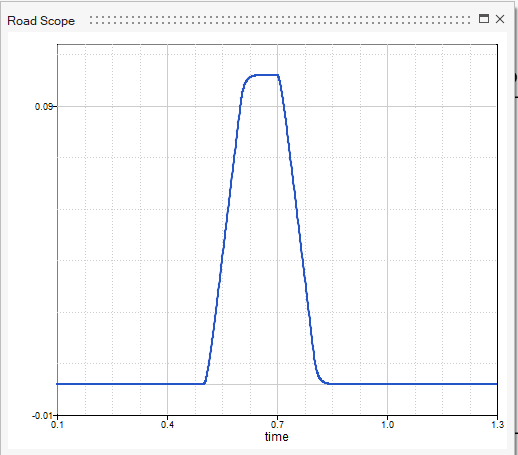
\includegraphics[width=.9\linewidth]{Pictures/big_bump_output.png}
  \caption{\emph{Road profile \#1 output}}
  %\captionof{figure}{Another figure}
  \label{fig:1bump_output}
\end{minipage}
\end{figure}
\subsubsection{profile \#2: realistic road profile}
A realistic road profile was created by steps: First of all we can think about it like a periodic function. The first approximation of this function is the sinusoidal waveform (the easiest one):
\begin{equation}
    h(t)=h_1 \sin(\omega t + \varphi)
\end{equation}
Of course, this is too simple to be realistic, so we can increase the road irregularity by adding more harmonics. The signal we obtain becomes:
\begin{equation}
    h(t)=h_1 \sin(\omega t + \varphi_1)+h_2 \sin(2\cdot\omega t + \varphi_2)+ \cdots + h_n \sin(n\cdot\omega t + \varphi_n)
\end{equation}
This approach is much more convenient than using a random number generator, because we can easily adjust $\omega$ and $h_i$ to simulate the car running on different terrains and speeds. Indeed, by knowing the speed of the car $v$, and the approximate length of the road bump $L$, we can obtain $\omega$ by using the following relation:
\begin{equation}
    \frac{2\pi v}{L}
\end{equation}
In the following table, you can find some statistical data for road irregularity length $L$, and amplitude $h_i$ that has been used to create the road signal.
\begin{table}[H]
    \centering
    \begin{tabular}{|l|c|c|}
         \hline
         \textbf{Road Type}& \textbf{$h_1$ [mm]} &	\textbf{L [m]}\\
         \hline
         \hline
         Motorway / Highway& 10 – 20 & 10 – 15\\
         \hline
         Urban roads (asphalt concrete)& 10 – 20 & 	1.0 – 2.0\\
         \hline
         Pavement roads (cobbles)& 30 – 40 & 0.15 – 0.30\\
         \hline
         Offroad& 50 – 70 & 0.10 – 0.15\\
         \hline
    \end{tabular}
    \caption{road irregularity length and amplitude\cite{road_profiles}}
    \label{tab:road_stats}
\end{table}
Once we have chosen $\omega$ and the various height $h_i$, we can increase the randomness of our output signal by choosing the various phases $\varphi_i$ in a random way: this mean that on each run of the simulation we will obtain a different road profile, but it's harmonic components will remains the same.
in \cref{fig:road_generator_sch} you can see the implementation on Altair Activate of this bump generator
\begin{figure}[H]
    \centering
    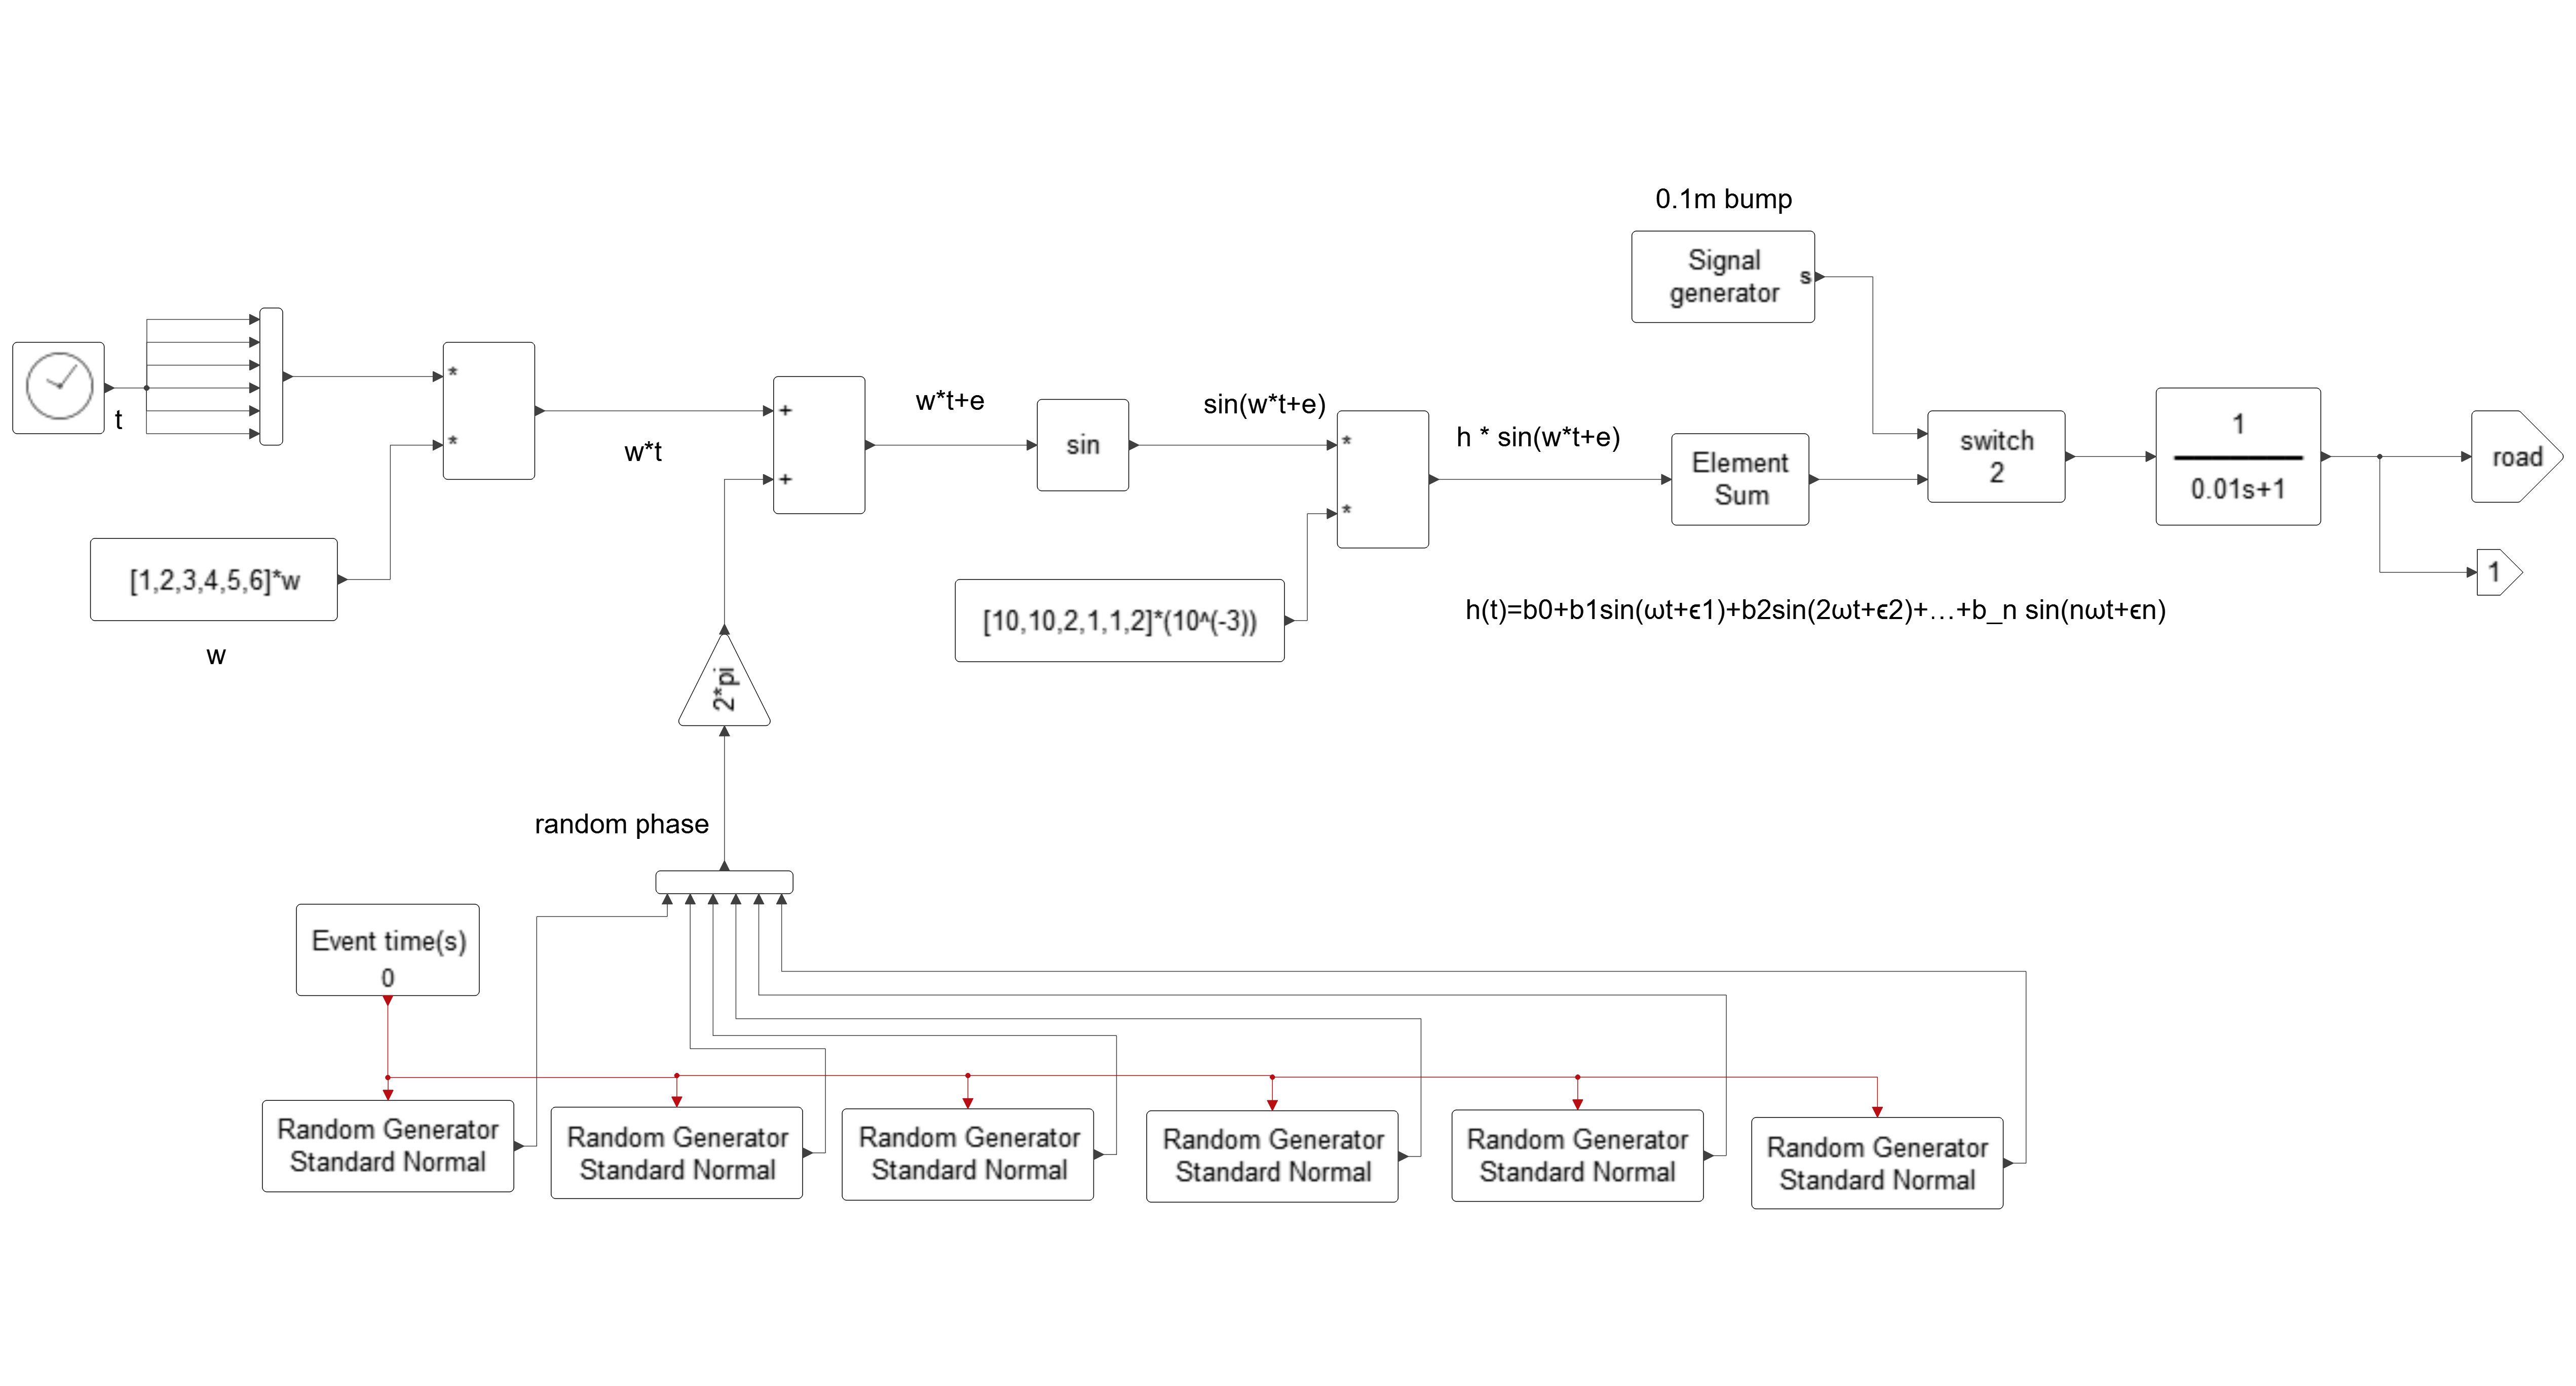
\includegraphics[width=0.99\textwidth]{Pictures/road_bump_generator.png}
    \caption{\emph{Road profile generator}}
    \label{fig:road_generator_sch}
\end{figure}
An example of urban road used in our simulations can be seen in \cref{fig:road_generator_example}, here the used parameters are:
\begin{itemize}
    \item $h_1=10$
    \item $v=\SI{50}{\kilo\metre/\hour}$
    \item $L=\SI{2}{\metre}$
\end{itemize}
\begin{figure}[H]
    \centering
    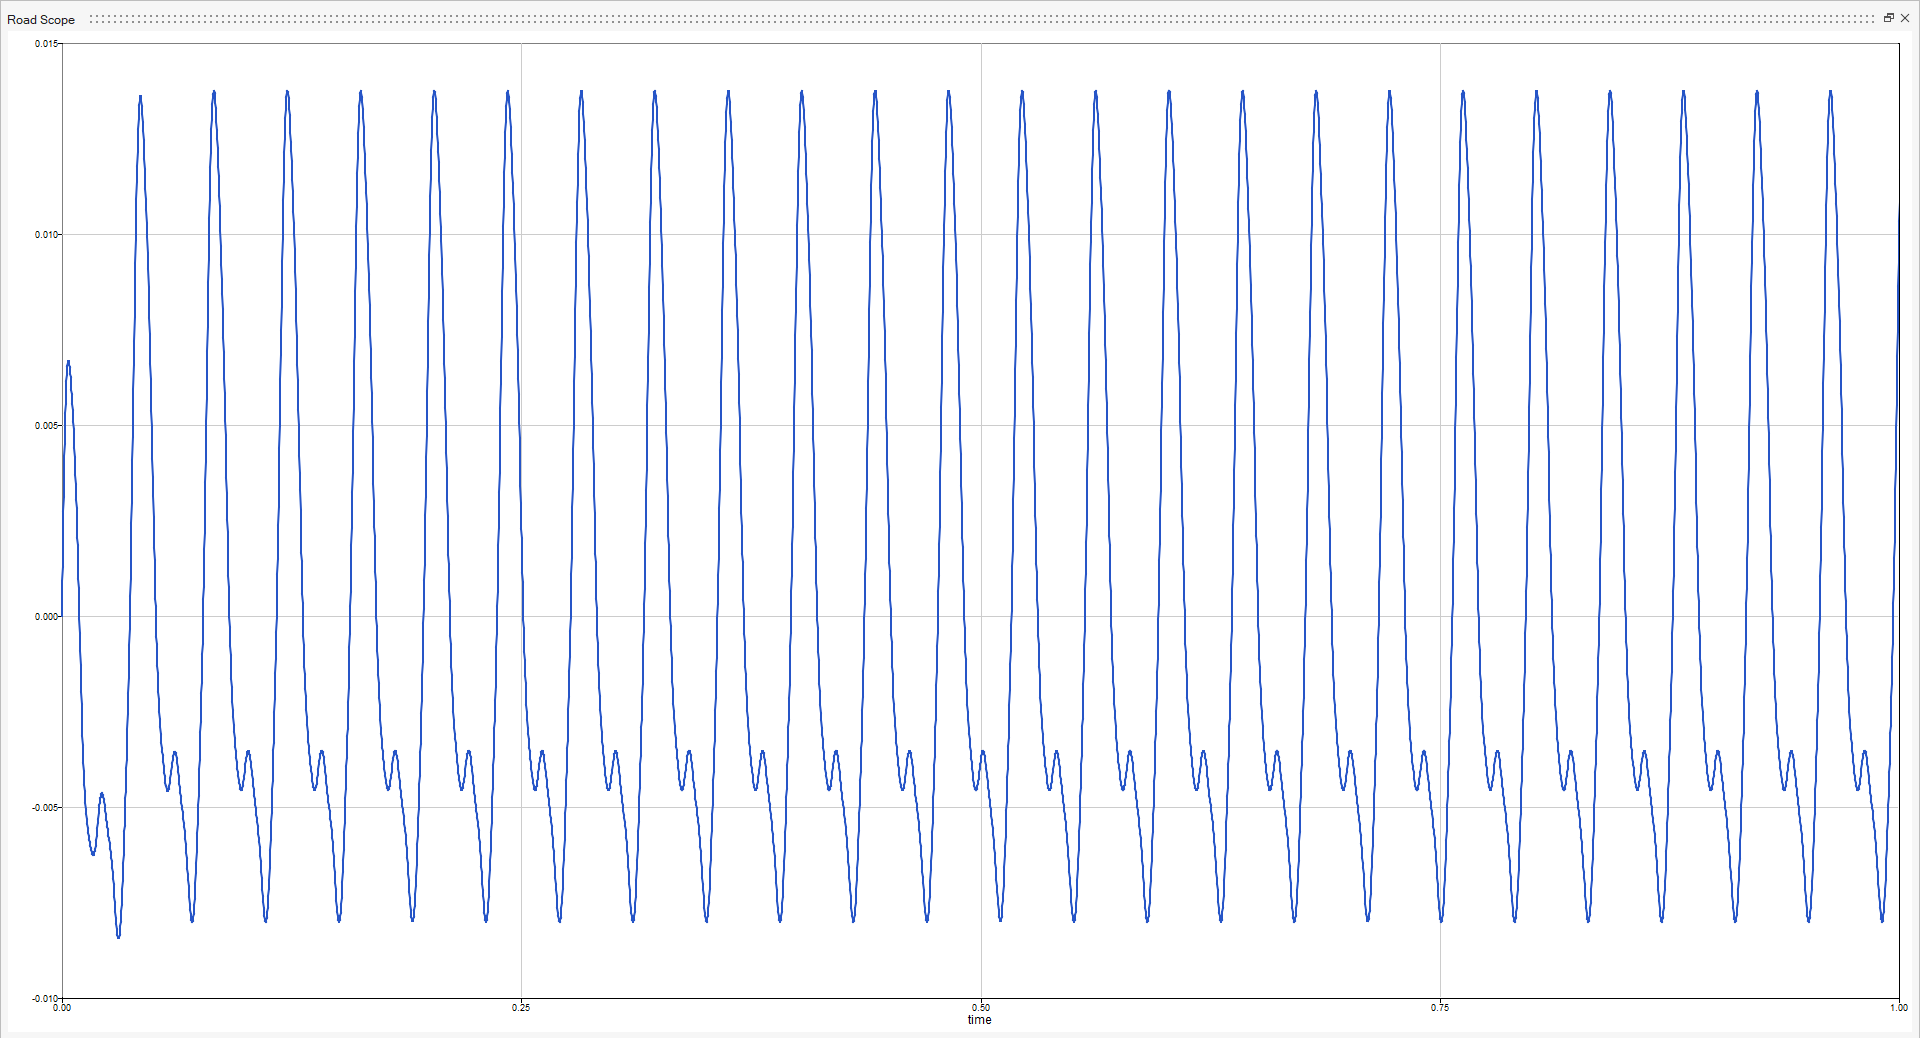
\includegraphics[width=0.9\textwidth]{Pictures/random_generated_road_profile.PNG}
    \caption{\emph{Road profile generated by our block}}
    \label{fig:road_generator_example}
\end{figure}
%By using a random generator, as can be seen in \cref{fig:road_generator_sch}, the road profile will be different at every run.
\subsection{Quarter car model}
The total vehicle mass is divided into two masses having only the vertical degree of freedom (2 DOF). The top mass represents the sprung part of the vehicle and its value is equal to the total weight of the sprung mass divided by 4. While, the second mass represents the unsprung part of the vehicle.\\
In between of the two masses we find the suspension that is modelled using a spring and a damper. In \cref{fig:5} the active suspension are implemented on the model using an actuator. The last components is the tire that in this model is represented with a spring to evaluate its stiffness. \\

\begin{figure}[H]
\centering
\begin{minipage}{.4\textwidth}
  \centering
  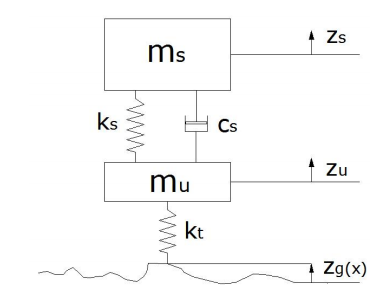
\includegraphics[width=.69\linewidth]{Pictures/quarter car.png}
  \caption{\emph{Passive suspension}}
  %\captionof{figure}{A figure}
  \label{fig:4}
\end{minipage}%
\begin{minipage}{.5\textwidth}
  \centering
  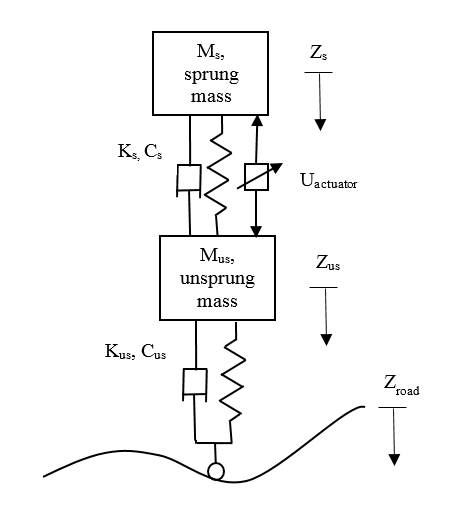
\includegraphics[width=.4\linewidth]{Pictures/quarter_car_diagram.PNG}
  \caption{\emph{Active suspension}}
  %\captionof{figure}{Another figure}
  \label{fig:5}
\end{minipage}
\end{figure}


\subsection{Model parameters}
In the following tables the parameters used in the simulation.\\
before to start, it is useful to know that the stiffness of the unsprung mass has been approximated by looking at various values found on literature \cite{article_stiffnes_tire}.\\
The stiffness and the dumping of the sprung mass have been seen during lectures, and then modified by using an optimization algorithm. 
\begin{table}[H]
\centering
\begin{tabular}{|l|c|}
\hline
\multicolumn{2}{|c|}{\textbf{FIAT 500e classic configuration}} \\ \hline
Sprung mass (ms) {[}kg{]}                     & 301            \\ \hline
Unsprung mass (mus) {[}kg{]}                  & 40             \\ \hline
Stiffness of unsprung (kus) {[}N/m{]}         & 200000         \\ \hline
Stiffness of sprung (ks) {[}N/m{]}            & 30000          \\ \hline
Dumping of unsprung (cus) {[}Ns/m{]}          & 0              \\ \hline
Dumping of sprung (cs) {[}Ns/m{]}             & 3000           \\ \hline
\end{tabular}\caption{\emph{Parameters of the classic FIAT 500e}}
\end{table}

\begin{equation}
    ms\_Classic=\frac{(TotalMass-(mus_C*4))}{4}
\end{equation}

\begin{table}[H]
\centering
\begin{tabular}{|l|c|}
\hline
\multicolumn{2}{|c|}{\textbf{FIAT 500e in-wheel configuration}} \\ \hline
Sprung mass (ms) {[}kg{]}                     & 271            \\ \hline
Unsprung mass (mus) {[}kg{]}                  & 73             \\ \hline
Stiffness of unsprung (kus) {[}N/m{]}         & 200000         \\ \hline
Stiffness of sprung (ks) {[}N/m{]}            & 30000          \\ \hline
Dumping of unsprung (cus) {[}Ns/m{]}          & 0              \\ \hline
Dumping of sprung (cs) {[}Ns/m{]}             & 3000           \\ \hline
\end{tabular}\caption{\emph{Parameters of the in-wheel FIAT 500e}}
\end{table}


\begin{equation}
    ms\_InWheel=\frac{(TotalMass-RemovedComponets)-(mus_I*2)-(mus_C*2)}{4}
    \label{eq:4.5}
\end{equation}


In the In-wheel configuration case, the approach used for the weight switch was the following.The weight of the unsprung mass increased by the weight of the motor. While, the weight of the sprung mass is reduced a little due to the absence of the motor and the transmission driveline (In \cref{eq:4.5}, these removed parts are called \emph{RemovedComponents}).\\ The total weight of the vehicle is reduced.\\


\subsection{Simulation: Passive suspension}
The stiffness and the dumping of the sprung mass have been tested with both the first profile, and the second road profile.\\
In \cref{fig:Passive comparison} is possible to notice the resulting acceleration in both the vehicles configuration equipped with the passive suspension. As expected, the acceleration in the case of the In-wheel car is higher and so the comfort for the passenger decrease.\\

\begin{figure}[H]
    \centering
    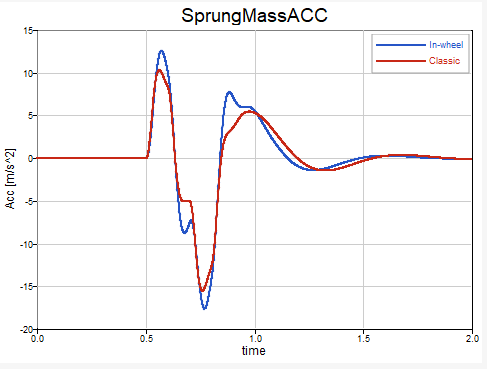
\includegraphics[width=0.5\textwidth]{Pictures/Passive (InWheelVsClassic).png}
    \caption{\emph{Acceleration comparison between classic and In-Wheel configuration}}
    \label{fig:Passive comparison}
\end{figure}

\subsubsection{Suspension optimization}

Those two values, Ks and cs, have been optimized by using an iterative optimization algorithm.
The algorithm used is the BobyqaOpt with the following parameters:
\begin{figure}[H]
    \centering
    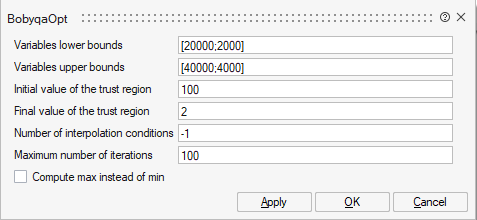
\includegraphics[width=0.5\textwidth]{Pictures/bobyaopt_param.PNG}
    \caption{\emph{BobyqaOpt block parameters for Ks and Cs}}
    \label{fig:bobyaopt_param}
\end{figure}
The road profile used is the second, but before to start we need to take in consideration the following:\\
If we remove the randomness of the initial phases of the road, the optimization algorithm will always converge to $Ks=0$ and $cs=0$, because the system will prefer to have a spring infinitely elastic, and a dumper with a non dumping behavior. Introducing the randomness of the phases, the results of the optimization are:
\begin{table}[H]
    \centering
    \begin{tabular}{|c|c|c|c|}
    \hline
         &no-optimization& classic opt. & in-wheel opt. \\
         \hline\hline
         \textbf{Ks}& $30e+3$ &$30e+3$ &$30e+3$\\
         \hline
         \textbf{cs}& $3.0e+3$ & $2.8e+3$ & $2.9e+3$\\
         \hline
    \end{tabular}
    \caption{Optimized Ks and Cs values}
    \label{tab:optimization_cs_ks}
\end{table}
We are aware that changing the road profile at every iteration is going to change the optimization function, and thus the results of \cref{tab:optimization_cs_ks} are not reliable, but the results didn't change much from the non optimized values and so we decided to use those.\\
Below, the results of the acceleration shows how the optimazed value of the suspension increase a little bit the performances of our system reducing the acceleration curve.
In \cref{fig:classic opt} the result for the classic FIAT 500e and in \cref{fig:InWheel opt} the acceleration plot for the In-wheel car.\\

\begin{figure}[H]
    \centering
    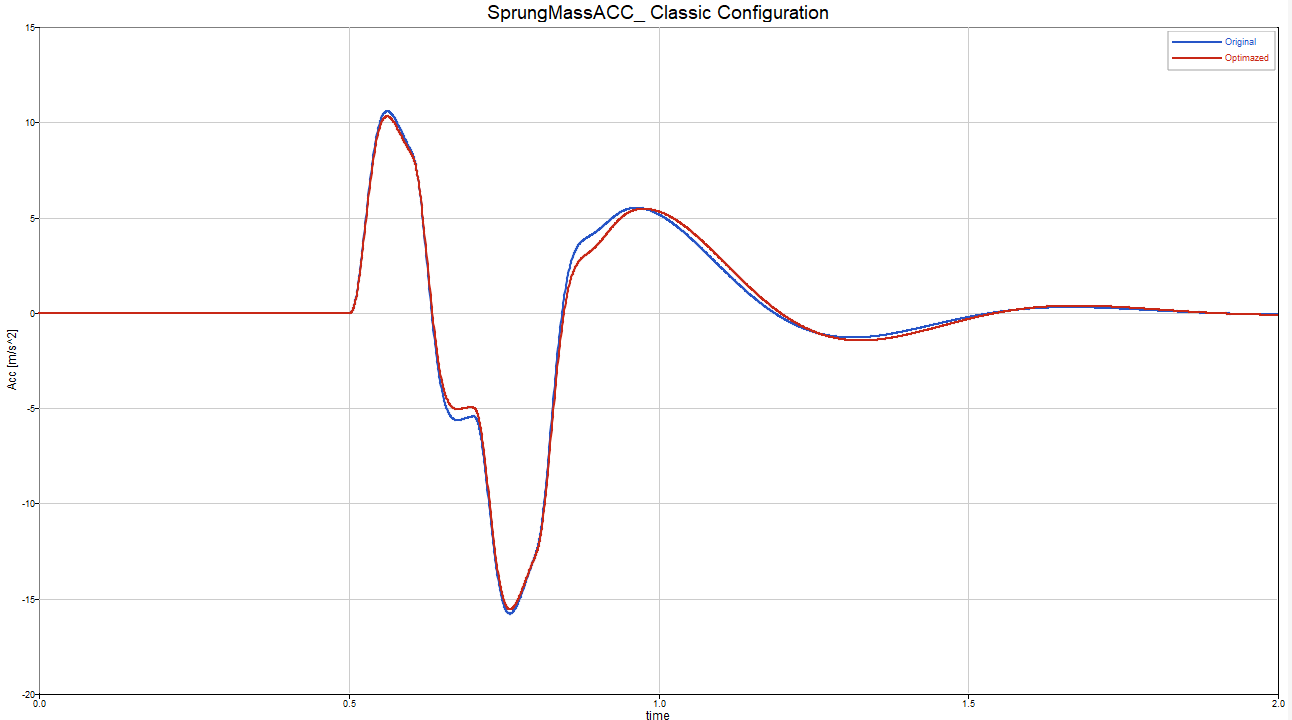
\includegraphics[width=0.6\textwidth]{Pictures/Passive (Classic Optimization).png}
    \caption{\emph{Acceleration with optimazed and non optimazed suspension (classic configuration)}}
    \label{fig:classic opt}
\end{figure}


\begin{figure}[H]
    \centering
    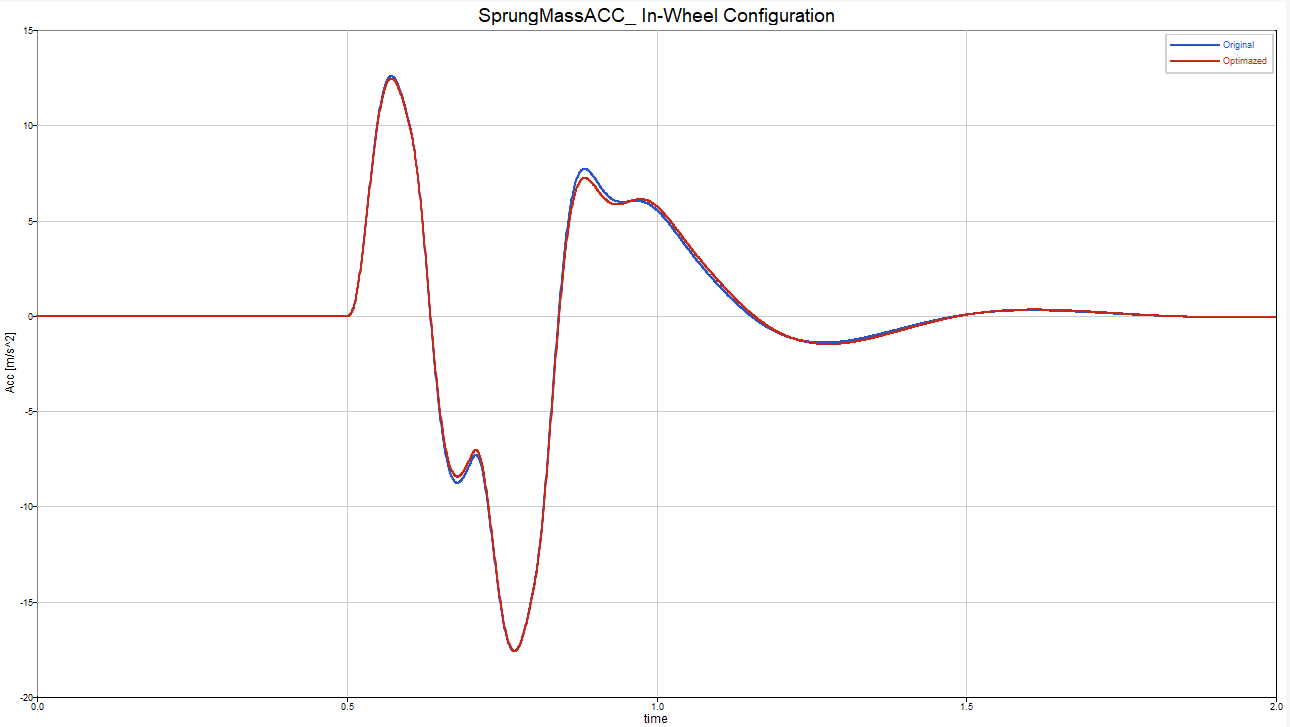
\includegraphics[width=0.6\textwidth]{Pictures/Passive (InWheel optimization).png}
    \caption{\emph{Acceleration with optimazed and non optimazed suspension (In-wheel configuration)}}
    \label{fig:InWheel opt}
\end{figure}
\subsection{Simulation: Active suspension}
The active suspensions are being introduced to increase the comfort of the driver and the passengers of the car. In our model, the active suspension are represented by a \emph{force acing on the suspension spring}. The force behavior can be changed by a PID controller, making it easy to be implemented and to be changed.

\begin{figure}[H]
    \centering
    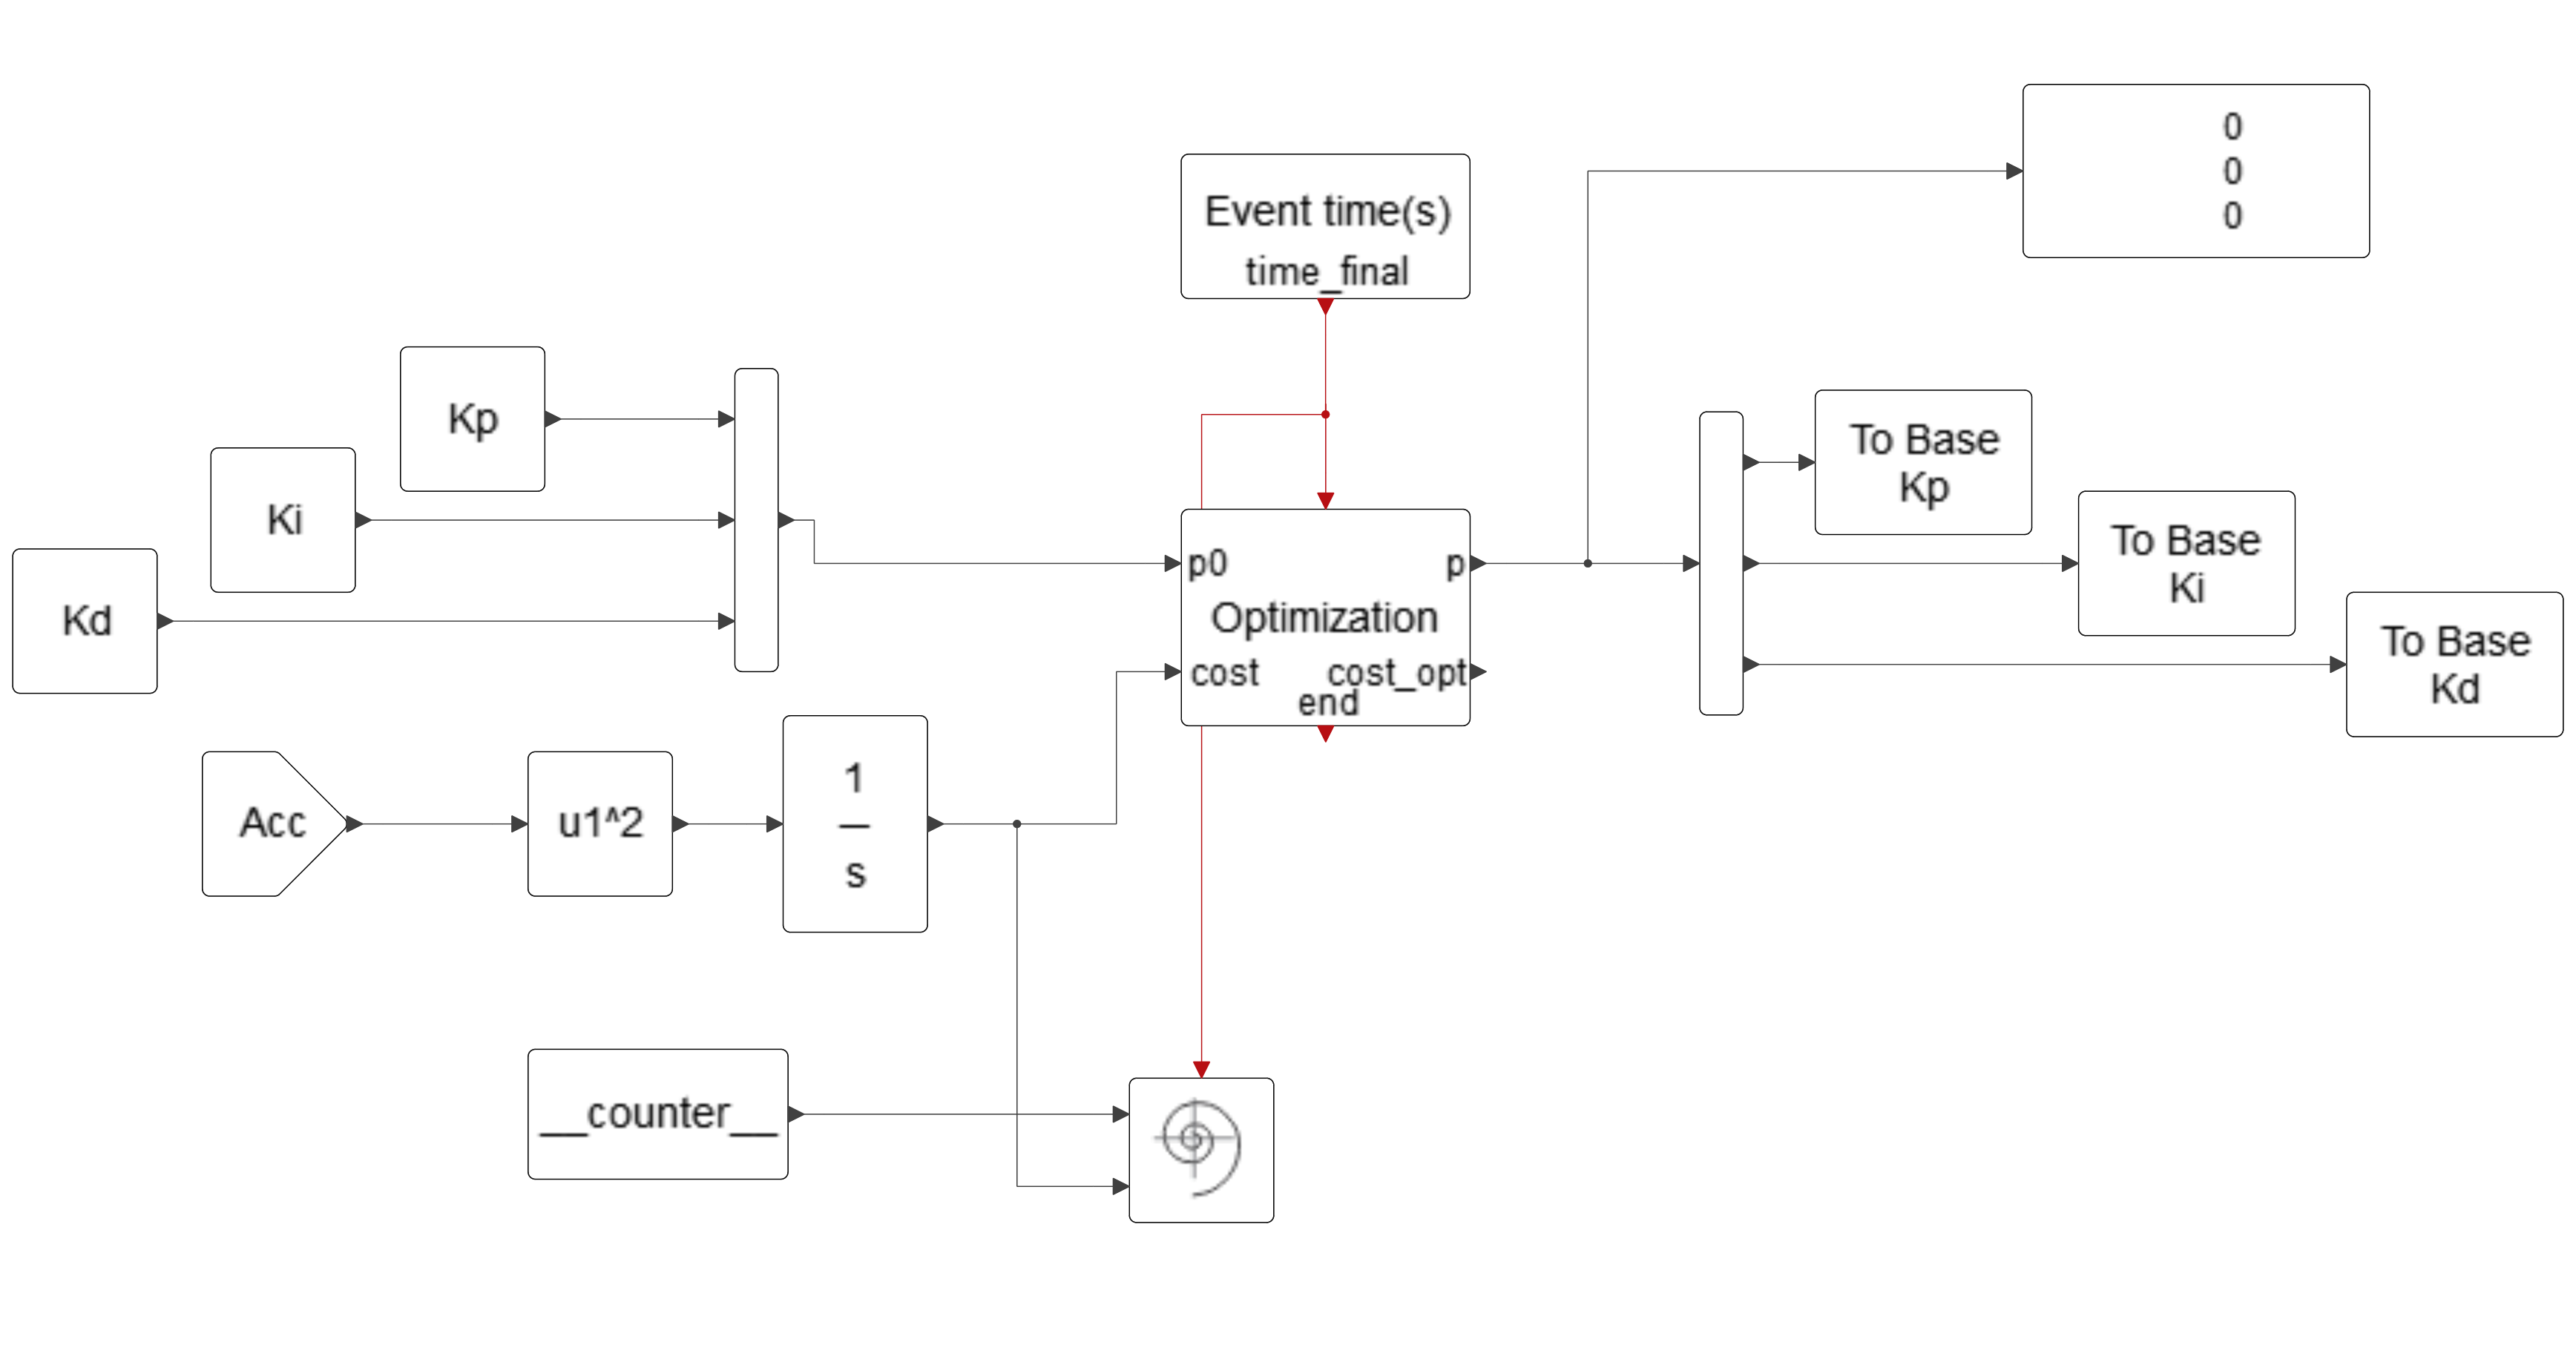
\includegraphics[width=0.6\textwidth]{Pictures/PID optimization.png}
    \caption{\emph{PID optimization}}
    \label{fig:PID algorithm}
\end{figure}
\subsubsection{PID optimization}
The PID parameters of the active suspension has being optimized by running the BobyqaOpt with the following parameters:
\begin{figure}[H]
    \centering
    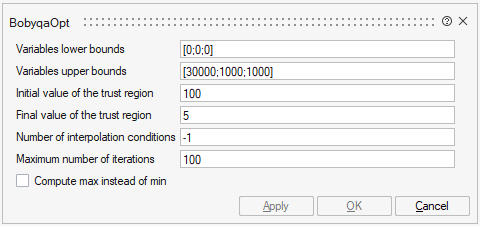
\includegraphics[width=0.5\textwidth]{Pictures/bobyapid.png}
    \caption{\emph{BobyqaOpt block parameters for PID}}
    \label{fig:bobyaopt_param_PID}
\end{figure}    
The road profile used is the first bump, and the results of the optimization are:
\begin{table}[H]
    \centering
    \begin{tabular}{|c|c|c|c|}
    \hline
         &no-optimization& classic opt. & in-wheel opt. \\
         \hline\hline
         \textbf{Kp}& $10e+3$ &$30e+3$ &$30e+3$\\
         \hline
         \textbf{Ki}& $0$ & $0$ & $0$\\
         \hline
         \textbf{Kd}& $0$ & $1e+3$ & $1e+3$\\
         \hline
    \end{tabular}
    \caption{Optimized PID values}
    \label{tab:optimization_PID}
\end{table}
The optimized PID values are the same between the In-wheel and classic car, but the result of the simulation looks quite different


\begin{figure}[H]
    \centering
    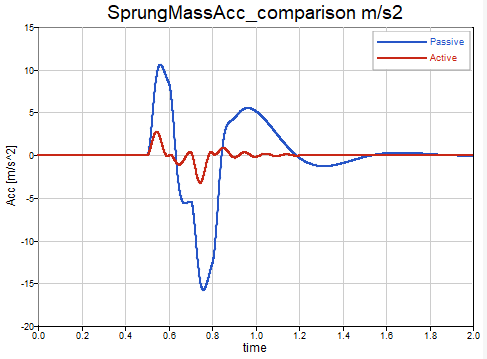
\includegraphics[width=0.6\textwidth]{Pictures/Active (classic configuration P30000 D1000).png}
    \caption{\emph{Acceleration for classic configuration with active suspension}}
    \label{fig:Classic PID}
\end{figure}

\begin{figure}[H]
    \centering
    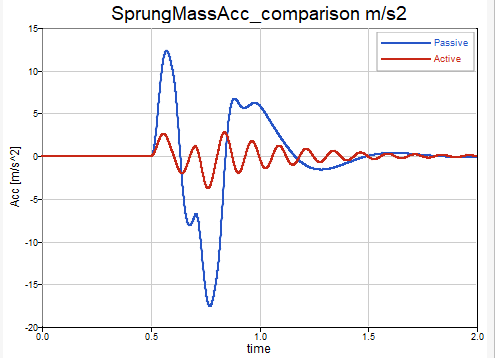
\includegraphics[width=0.6\textwidth]{Pictures/Active (In wheel configuration P30000 D1000).png}
    \caption{\emph{Acceleration for In-Wheel configuration with active suspension}}
    \label{fig:InWheel PID}
\end{figure}
\section{Conclusions}
The aim of this project was to see how the unsprung mass would affect the comfort on our system: we can notice that with a passive solution the two system behave nearly the same (the maximum vertical acceleration of the In-wheel configuration is higher, but not that much, see \cref{fig:Passive comparison}). In order to understand how much this increase of acceleration affects the comfort further investigation should be done.
On the other side, applying an active suspension seems to be very effective for both the configuration. Here we can clearly see how an high unsprung mass could affect the car vertical dynamics, and thus the comfort of the driver: The In-Wheel configuration suffers by more pronounced spikes, and a longer transient.\\
Even if those problem does looks tedious, the great advantage of having less total car weight could become a key factor for new EVs generations, so we can speculate that a good amount of research interest is going to be spent on that field.
%%%%%%%%%%%%%%%%%%%%%
\newpage

\bibliographystyle{unsrt}
\bibliography{sample}

\end{document}